\documentclass[11pt]{article}


% Use wide margins, but not quite so wide as fullpage.sty
\marginparwidth 0.5in 
\oddsidemargin 0.25in 
\evensidemargin 0.25in 
\marginparsep 0.25in
\topmargin 0.25in 
\textwidth 6in \textheight 8 in

\usepackage{hyperref}
\usepackage{siunitx}

% To load schematic diagram, we would need graphicx
\usepackage{graphicx}
\graphicspath{ {images/} }


\begin{document}
\author{Rahul Jha, Atiya Fatima Usmani and Umamah Khan}
\title{Assignment: IC-741 Simulation}
\maketitle

\section{Synopsis}
Operating Point, Transient and AC analysis of the IC-741 circuit were performed in simulation using LTSpice XVII.
\newpage

\section{Schematic}
The following schematic was used to carry out the simulation process:
\newline

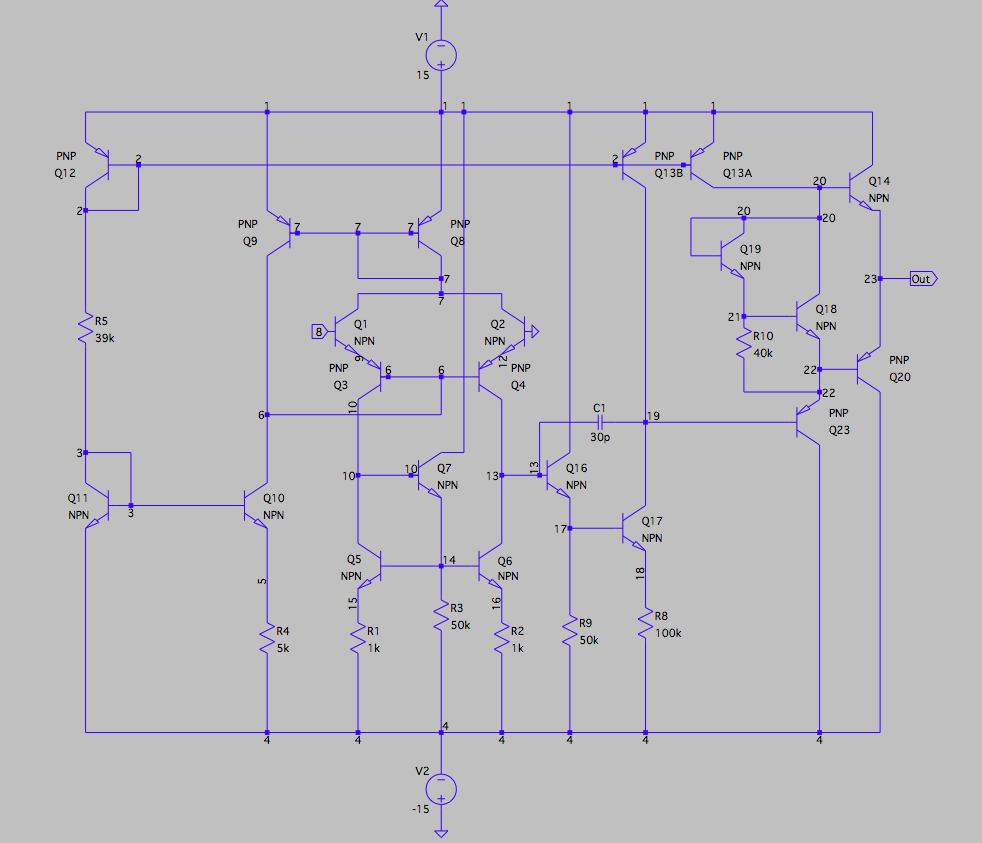
\includegraphics[width=\textwidth]{Schematic.png}

\section{Netlist}
Using the above schematic, the following netlist was prepared:

\begin{verbatim}
* Simulation of IC-741 OpAmp
* Authors: Rahul Jha, Atiya Fatima Usmani and Umamah Khan
* Biasing:
V+ 1 0 15
V- 0 4 15
* Input Sine:
Vi 8 0 AC 0.5 sin(0 0.5 1khz)
* Circuit:
Q1 7 8 9 0 Q2N3904
Q2 7 0 12 0 Q2N3904
Q3 10 6 9 0 Q2N3906
Q4 13 6 12 0 Q2N3906
Q5 10 14 15 0 Q2N3904
Q6 13 14 16 0 Q2N3904
Q7 1 10 14 0 Q2N3904
Q8 7 7 1 0 Q2N3906
Q9 6 7 1 0 Q2N3906
Q10 6 3 5 0 Q2N3904
Q11 3 3 4 0 Q2N3904
Q12 2 2 1 0 Q2N3906
Q13A 20 2 1 0 Q2N3906 0.25
Q13B 19 2 1 0 Q2N3906 0.75
Q18 20 21 22 0 Q2N3904
Q19 20 20 21 0 Q2N3904
Q14 1 20 23 0 Q2N3904 20
Q20 4 22 23 0 Q2N3906 20
Q23 4 19 22 0 Q2N3906
Q16 1 13 17 0 Q2N3904
Q17 19 17 18 0 Q2N3904
R1 15 4 1k
R2 16 4 1k
R3 14 4 50k
R4 5 4 5k
R5 2 3 39k
R8 18 4 100
R9 17 4 150k
R10 21 22 40k
Cc 19 13 30p
.model Q2N3904 NPN(Is=6.734f Xti=3 Eg=1.11 Vaf=74.03 Bf=416.4 Ne=1.259
+ Ise=6.734f Ikf=66.78m Xtb=1.5 Br=.7371 Nc=2 Isc=0 Ikr=0 Rc=1
+ Cjc=3.638p Mjc=.3085 Vjc=.75 Fc=.5 Cje=4.493p Mje=.2593 Vje=.75
+ Tr=239.5n Tf=301.2p Itf=.4 Vtf=4 Xtf=2 Rb=10)
.model Q2N3906 PNP(Is=1.41f Xti=3 Eg=1.11 Vaf=18.7 Bf=180.7 Ne=1.5 Ise=0
+ Ikf=80m Xtb=1.5 Br=4.977 Nc=2 Isc=0 Ikr=0 Rc=2.5 Cjc=9.728p
+ Mjc=.5776 Vjc=.75 Fc=.5 Cje=8.063p Mje=.3677 Vje=.75 Tr=33.42n
+ Tf=179.3p Itf=.4 Vtf=4 Xtf=6 Rb=10)
.end
\end{verbatim}

\section{Operating Point Analysis}
The result of .op analysis is as follows:
\begin{verbatim}
V(1):	 15	 voltage
V(4):	 -15	 voltage
V(8):	 0	 voltage
V(7):	 14.4118	 voltage
V(9):	 -0.525551	 voltage
V(12):	 -0.525484	 voltage
V(10):	 -13.9253	 voltage
V(6):	 -1.08292	 voltage
V(13):	 -13.7622	 voltage
V(14):	 -14.4649	 voltage
V(15):	 -14.9946	 voltage
V(16):	 -14.9946	 voltage
V(3):	 -14.3425	 voltage
V(5):	 -14.9017	 voltage
V(2):	 14.3022	 voltage
V(20):	 14.2051	 voltage
V(19):	 12.3909	 voltage
V(21):	 13.6455	 voltage
V(22):	 13.0283	 voltage
V(23):	 13.6253	 voltage
V(17):	 -14.2951	 voltage
V(18):	 -14.9395	 voltage
Ic(Q23):	 -0.000174772	 device_current
Ib(Q23):	 -3.92734e-007	 device_current
Ie(Q23):	 0.000175164	 device_current
Ic(Q20):	 -0.000745865	 device_current
Ib(Q20):	 -1.65211e-006	 device_current
Ie(Q20):	 0.000747518	 device_current
Ic(Q13b):	 -0.000600455	 device_current
Ib(Q13b):	 -3.04247e-006	 device_current
Ie(Q13b):	 0.000603498	 device_current
Ic(Q13a):	 -0.000182535	 device_current
Ib(Q13a):	 -1.01416e-006	 device_current
Ie(Q13a):	 0.000183549	 device_current
Ic(Q12):	 -0.000726367	 device_current
Ib(Q12):	 -4.05662e-006	 device_current
Ie(Q12):	 0.000730423	 device_current
Ic(Q9):	 -1.93972e-005	 device_current
Ib(Q9):	 -5.86963e-008	 device_current
Ie(Q9):	 1.94559e-005	 device_current
Ic(Q8):	 -1.06077e-005	 device_current
Ib(Q8):	 -5.87118e-008	 device_current
Ie(Q8):	 1.06664e-005	 device_current
Ic(Q4):	 -5.41713e-006	 device_current
Ib(Q4):	 -1.78539e-008	 device_current
Ie(Q4):	 5.43498e-006	 device_current
Ic(Q3):	 -5.43122e-006	 device_current
Ib(Q3):	 -1.78075e-008	 device_current
Ie(Q3):	 5.44903e-006	 device_current
Ic(Q17):	 0.000600848	 device_current
Ib(Q17):	 3.71082e-006	 device_current
Ie(Q17):	 -0.000604559	 device_current
Ic(Q16):	 8.3093e-006	 device_current
Ib(Q16):	 1.00666e-007	 device_current
Ie(Q16):	 -8.40997e-006	 device_current
Ic(Q14):	 0.000738495	 device_current
Ib(Q14):	 9.02251e-006	 device_current
Ie(Q14):	 -0.000747518	 device_current
Ic(Q19):	 1.67192e-005	 device_current
Ib(Q19):	 2.3541e-007	 device_current
Ie(Q19):	 -1.69546e-005	 device_current
Ic(Q18):	 0.000156558	 device_current
Ib(Q18):	 1.52302e-006	 device_current
Ie(Q18):	 -0.000158081	 device_current
Ic(Q11):	 0.000728532	 device_current
Ib(Q11):	 5.71561e-006	 device_current
Ie(Q11):	 -0.000734247	 device_current
Ic(Q10):	 1.94328e-005	 device_current
Ib(Q10):	 2.3261e-007	 device_current
Ie(Q10):	 -1.96654e-005	 device_current
Ic(Q7):	 1.07581e-005	 device_current
Ib(Q7):	 1.24397e-007	 device_current
Ie(Q7):	 -1.08825e-005	 device_current
Ic(Q6):	 5.31646e-006	 device_current
Ib(Q6):	 9.06383e-008	 device_current
Ie(Q6):	 -5.4071e-006	 device_current
Ic(Q5):	 5.30683e-006	 device_current
Ib(Q5):	 9.06662e-008	 device_current
Ie(Q5):	 -5.39749e-006	 device_current
Ic(Q2):	 5.35561e-006	 device_current
Ib(Q2):	 7.93749e-008	 device_current
Ie(Q2):	 -5.43498e-006	 device_current
Ic(Q1):	 5.36949e-006	 device_current
Ib(Q1):	 7.95441e-008	 device_current
Ie(Q1):	 -5.44903e-006	 device_current
I(Cc):	 7.84592e-022	 device_current
I(R10):	 1.54316e-005	 device_current
I(R9):	 4.69915e-006	 device_current
I(R8):	 0.000604559	 device_current
I(R5):	 0.00073448	 device_current
I(R4):	 1.96654e-005	 device_current
I(R3):	 1.07012e-005	 device_current
I(R2):	 5.4071e-006	 device_current
I(R1):	 5.39749e-006	 device_current
I(Vi):	 -7.95441e-008	 device_current
I(V-):	 -0.00230531	 device_current
I(V+):	 -0.00230515	 device_current
\end{verbatim}
\newpage
\section{Transient Analysis}
The following directive was added to the netlist to perform the transient analysis:
\begin{verbatim}
    .tran 10m
\end{verbatim}
The following plot was observed:
\newline

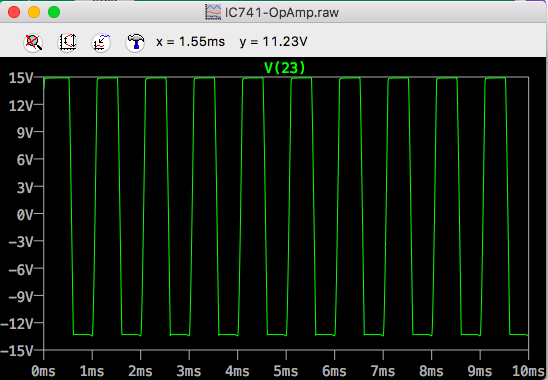
\includegraphics[width=\textwidth]{Transient.png}

\pagebreak

\section{AC Analysis}
The following spice directive was added:

\begin{verbatim}
    .ac dec 100 1 10k
\end{verbatim}

Plot observed:
\newline

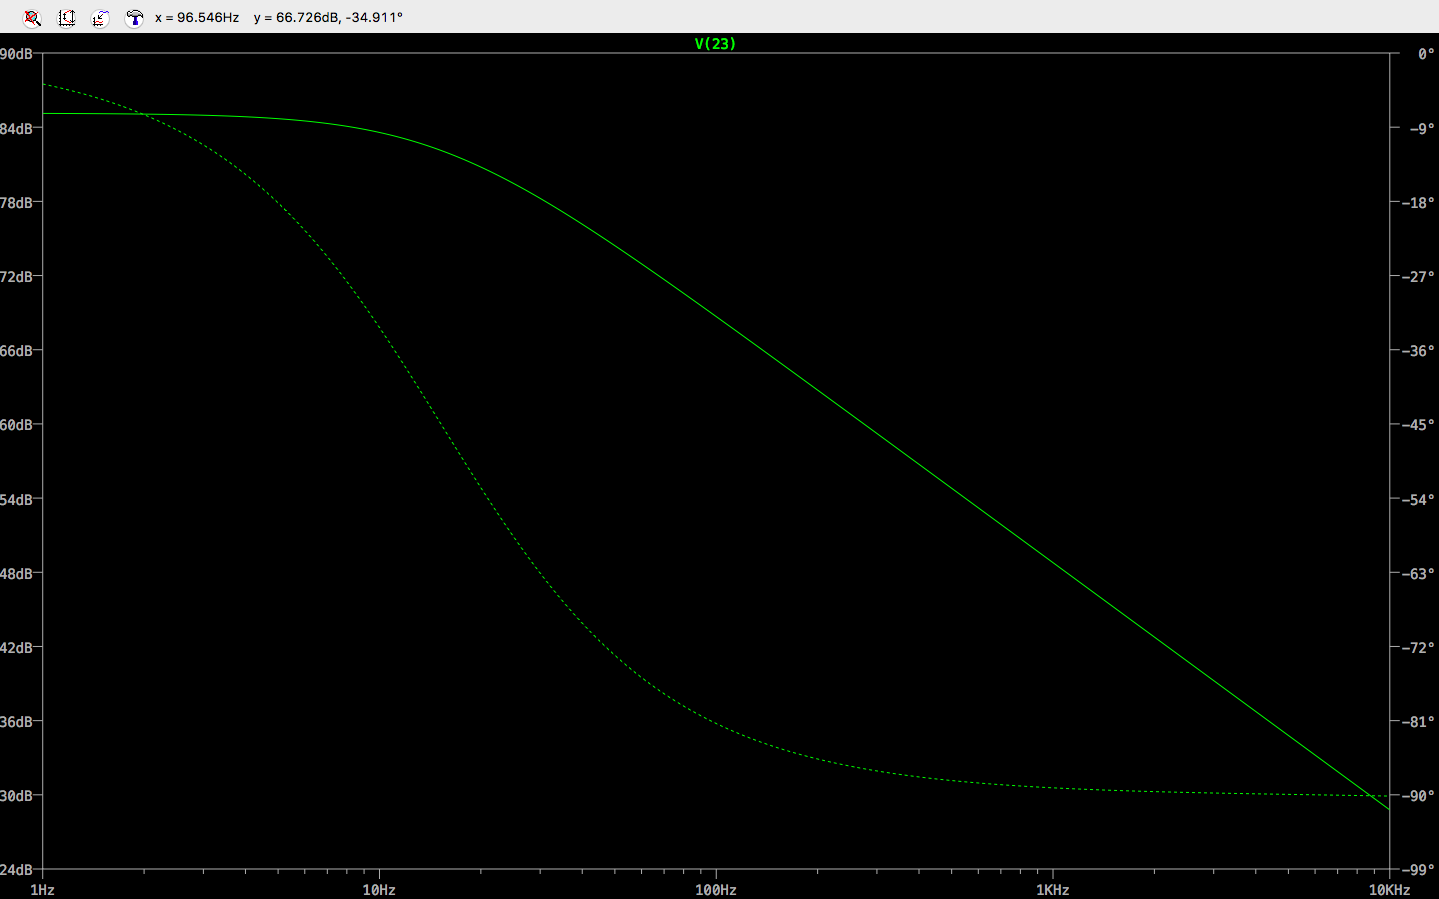
\includegraphics[width=\textwidth]{AC_150.png}

\newpage

\textbf{Note:} R9 was increased to a value of 150K, otherwise the plot was distorted:
\newline

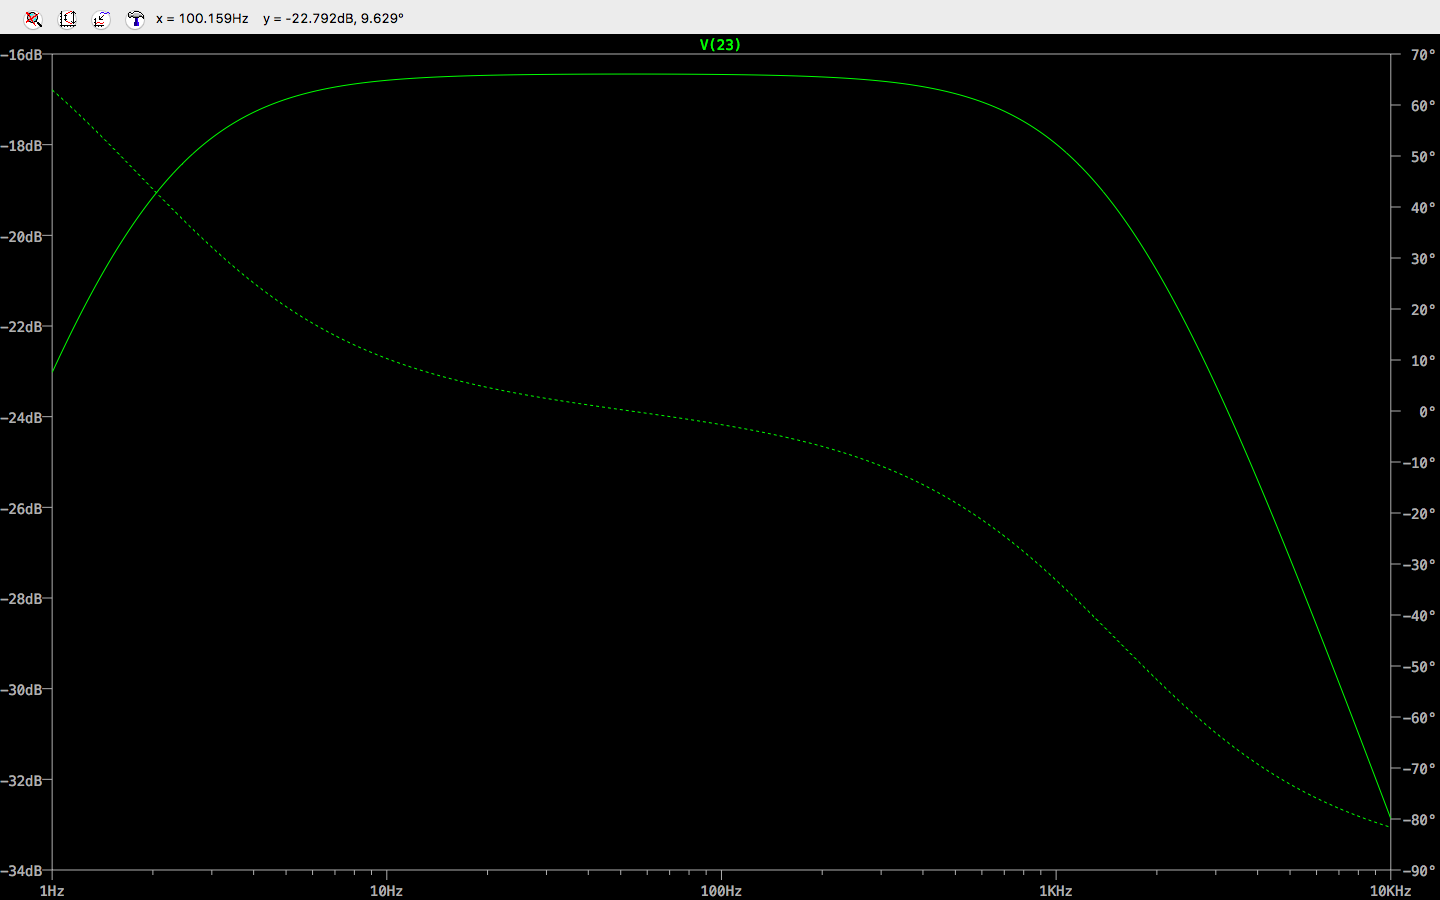
\includegraphics[width=\textwidth]{AC_50.png}

\section{Comparison}
\begin{center}
\begin{tabular}{ c c c }
 Transistor & Calculated Value(\SI{}{\micro}A) & Spice Value(\SI{}{\micro}A) \\
 Q1 & 9.5 & 5.36 \\
 Q2 & 9.5 & 5.35 \\
 Q3 & 9.5 & 5.43 \\
 Q4 & 9.5 & 5.41 \\
 Q5 & 9.5 & 5.30 \\
 Q6 & 9.5 & 5.31 \\
 Q7 & 10.5 & 10.7 \\
 Q8 & 19 & 10.6 \\
 Q9 & 19 & 19.3 \\
 Q10 & 19 & 19.4 \\
 Q11 & 730 & 728 \\
 Q12 & 730 & 726 \\
 Q13A & 180 & 182.5 \\
 Q13B & 550 & 600.4 \\
 Q14 & 154 & 113.7 \\
 Q16 & 16.2 & 8.3 \\
 Q17 & 550 & 600 \\
 Q18 & 165 & 164 \\
 Q19 & 15.8 & 16.8 \\
 Q20 & 154 & 114.8 \\
 Q23 & 180 & 174.7 \\
\end{tabular}
\end{center}

\section{Citations}
Models Q2N3904 \& Q2N3906 are a courtesy of \href{http://ece.utah.edu/~ccharles/ece3110/Labs/spice_models.html}{ece.utah.edu}

\end{document}
